\documentclass[11pt,a4paper]{article}
\usepackage[a4paper,margin=2.5cm]{geometry}
\usepackage{graphicx}
\usepackage{booktabs}
\usepackage{amsmath}
\usepackage{float}
\usepackage{caption}
\usepackage{subcaption}
\usepackage{siunitx}
\usepackage[hidelinks]{hyperref}

\setlength{\parskip}{0.5em}
\setlength{\parindent}{0pt}
\renewcommand{\baselinestretch}{1.15}

\begin{document}

% Title
\begin{titlepage}
\centering
\vspace*{7cm}
{\LARGE \textbf{Reinforcement Learning for Sepsis Treatment Optimization}}\\[0.5cm]
{\large Policy Learning in Discrete and Continuous Clinical Environments}\\[10cm]
\textbf{Authors:} Andreea Roica, Marisa Esteves, Miguel Caramelo, Oliver Kain \\
\textbf{Student IDs:} 20250361, 20250348, 20250378, 20250401 \\
\textbf{Professor:} Inês Castelhano\\
\textbf{Course:} Reinforcement Learning \\
\textbf{University:} NOVA Information Management School \\
\textbf{Date:} June 05, 2026
\vfill
\end{titlepage}

% Table of Contents
\tableofcontents
\clearpage

\section{Abstract (optional)}
Short summary: problem motivation (sepsis treatment), RL approach, config A vs config B, algorithms used, main findings, 
creative extension contribution.

\section{Introduction}

Sepsis is one of the leading causes of mortality in intensive care units (ICUs) worldwide and represents a major challenge in modern healthcare. 
The condition arises from the body’s dysregulated response to infection, often leading to organ failure and severe physiological instability.
Treating sepsis requires clinicians to continuously make complex decisions regarding intravenous (IV) fluids and vasopressor administration 
in order to stabilize the patient while avoiding harmful side effects caused by excessive treatment. 
Because patient responses vary significantly and outcomes are often delayed, determining the optimal treatment strategy is highly challenging.

This setting naturally motivates the application of Reinforcement Learning (RL).
In the context of sepsis treatment, the RL agent learns treatment policies directly from historical ICU trajectories, 
aiming to maximize patient survival while minimizing unnecessary interventions.

In this project, we investigate the application of RL methods to the ICU-Sepsis-v2 benchmark environment,
which is derived from the real-world MIMIC-III clinical database. 
The project is divided into two distinct configurations that reflect different levels of environmental complexity. 
Configuration A uses a discrete state representation, allowing the application of classical tabular reinforcement learning methods 
and model-based approaches. Configuration B introduces a continuous high-dimensional observation space composed of physiological measurements,
requiring the use of deep reinforcement learning and function approximation techniques.

The primary objective of this work is to compare the behavior and performance of reinforcement learning algorithms across both environments.

To extend the analysis, we developed a creative extension focused on policy agreement and ensemble behavior. 
By analyzing agreement and disagreement patterns between learned policies, 
we aim to better understand uncertainty and robustness in clinical decision-making scenarios.

\section{Environment and Problem Setup}
The experiments were conducted using the ICU-Sepsis-v2 environment, 
a benchmark designed for offline reinforcement learning in healthcare applications. 
The environment is based on patient trajectories extracted from the MIMIC-III clinical database 
and simulates the treatment of sepsis patients in intensive care units. 
Each episode corresponds to a single patient trajectory, 
where the agent sequentially observes the patient’s condition and selects a treatment action at every timestep.

The action space is discrete and composed of 25 possible actions, 
representing combinations of vasopressor dosage and IV fluid administration levels.
The objective of the agent is to learn a treatment policy that maximizes patient survival outcomes. 
At the end of each episode, the agent receives a terminal reward of +1 if the patient survives and 0 otherwise.


\subsection{Configuration A: Discrete State Space}
In Configuration A, the environment provides a discrete representation of the patient state. 
Each observation corresponds to an integer between 0 and 715, 
resulting in a finite state space of 716 possible clinical states. 
Since both the state and action spaces are discrete and relatively small, 
classical tabular reinforcement learning methods become computationally feasible.
In particular, 
the complete transition and reward matrices of the underlying Markov Decision Process (MDP) are accessible, 
enabling the use of model-based algorithms.

To better understand the environment before training the agents, 
an exploratory analysis of the MDP structure was conducted. 
The transition dynamics were relatively sparse, 
with only around 12\% of all possible state-action-next-state transitions having non-zero probability. 
However, the environment exhibited substantial stochasticity and uncertainty. 
On average, each state-action pair could transition to approximately 85 possible next states, 
indicating a high branching factor and variability in patient outcomes following 
identical clinical interventions.

The reward structure of the environment is sparse and primarily terminal-based.
Although most states are connected to at least some positive reward signal (687 states), 
the average expected reward per state remains low (0.1133), 
suggesting that survival signal is widely reachable across the state space
but remains weak and unevenly distributed.

Additional analysis of the reward matrix revealed that approximately 72\% of states 
contain a clearly dominant action with the highest expected reward.
However, the distribution of optimal actions across states was highly imbalanced, 
with some actions appearing optimal far more frequently than others (Figure \ref{app:fig:best_actions}).

A random-policy baseline was also evaluated in order to establish a minimum performance threshold
for the learning agents. It provided a reference point for determining whether the learned agents
extract meaningful treatment strategies beyond random exploration.


\subsection{Configuration B: Continuous Observation Space}
- 47-dimensional physiological vector, need for function approximation, challenges of continuous observations

\section{Methodology}
\subsection{Evaluation Metrics}
Explain: average return, success/ survival rate, convergence speed, stability/ variance, exploration behavior

\subsection{Configuration A Algorithms}

\subsubsection{Policy Iteration}
Core idea, why appropriate for config A, update equations (briefly), hyperparameters.

\subsubsection{Value Iteration}
Core idea, differences from policy iteration, update equations (briefly), hyperparameters.

\subsubsection{Training Setup}
Episodes, seeds, discount factor, learning rate, epsilon-decay, etc.

\subsection{Configuration B Algorithms}
\subsubsection{Double DQN}
Neural network architecture, replay buffer/ policy updates, why chosen for continuous observations

\subsubsection{PPO}
Policy gradient method, why chosen for continuous actions

\subsubsection{Training Setup}
Architecture, batch size, optimizer, learning schedule, hardware/runtime considerations.

\section{Results and Evaluation}
Figures and analysis.

\subsection{Configuration A Results}
\subsubsection{Training Curves}
Reward Evolution, convergence plots.

\subsubsection{Performance Comparison}
Results table, stability analysis, exploration vs exploitation discussion.

\subsubsection{Policy Interpretation}
Which actions are preferred, clinical interpretation, interesting patterns.

\subsection{Configuration B Results}
\subsubsection{Training Curves}
\subsubsection{Performance Comparison}
\subsubsection{Deep RL Behavior Analysis}
Learning stability, sample efficiency, generalization observations.

\subsection{Config A vs Config B Comparison}
Include comparison table, tabular RL vs deep RL, computational complexity, interpretability, stability, state representation differences,
when deep RL becomes necessary.

\section{Creative Extension: Policy Agreement \& Ensemble Analysis}
\subsection{Motivation}
As a creative extension, we explored policy agreement and ensemble decision-making in the continuous observation setting of Configuration B. 
While RL agents are commonly evaluated using aggregate performance metrics such as mean return or survival rate, 
these metrics provide limited insight into how different agents behave internally or whether they learn similar treatment strategies.

In clinical applications, robustness and consistency are particularly important. 
Two agents with comparable performance may still recommend substantially different treatments for the same patient state, 
raising questions regarding reliability and interpretability. 
Therefore, this extension aimed to investigate whether different RL algorithms converge toward similar clinical decisions 
and whether policy disagreement could be leveraged through ensemble methods to improve performance.

We hypothesized that agreement between agents would be higher in stable or low-severity patient states and lower in uncertain or clinically severe situations.
Additionally, we expected that combining complementary behaviors from different policies through ensemble strategies could improve robustness
and overall decision quality.

\subsection{Method}
After training both the Double DQN and PPO agents, 
evaluation trajectories were collected from each policy using identical episode seeds 
to ensure that both agents were evaluated under comparable clinical conditions. 
For every timestep, the stored information included the patient observation, 
SOFA severity score, selected action from each policy, action confidence scores, 
and indicators for noisy episodes or missing observations.

Policy agreement was defined as the percentage of timesteps in which both agents selected the same action. 
Agreement rates were analyzed globally and across different SOFA severity groups. 
To further study policy behavior throughout patient trajectories, 
episodes were divided into early and late phases, allowing agreement rates to be compared over time.

Disagreement analysis was then performed by identifying the most frequent disagreement 
action pairs between PPO and DDQN. 
Additional comparisons examined whether disagreement was associated with patient severity, 
noisy episodes, or missing observations.

Finally, two ensemble policies were implemented. 
Ensemble A followed a simple agreement-and-tie-break strategy: if both agents selected the same action, 
that action was executed; otherwise, the decision defaulted to a designated tie-break agent. 
Ensemble B implemented a confidence-based arbitration mechanism, selecting the action proposed by the agent with the highest confidence score. 
PPO confidence was obtained directly from policy probabilities, while DDQN confidence was approximated using a softmax transformation 
of the Q-values in order to place both confidence measures on a comparable scale.

\subsection{Results and Discussion}
The agreement analysis revealed extremely low policy agreement between DDQN and PPO. 
Across more than 17,000 evaluated timesteps, the agents selected the same action in only approximately 4\% of states, 
indicating that they learned substantially different treatment strategies despite being trained in the same environment.

Contrary to the initial expectation, agreement remained consistently low across all SOFA severity groups (3.7\%–4.5\%),
suggesting that disagreement was not strongly associated with patient severity (Figure \ref{app:fig:policy_agreement_ensemble_analysis}).
A small increase in agreement was observed during later episode stages, 
indicating that the agents may converge slightly more frequently as patient trajectories progress.

The disagreement analysis highlighted clear behavioral differences between the agents. 
PPO strongly concentrated its policy around a small subset of actions, particularly action 5, 
which accounted for more than 60\% of selections. 
In contrast, DDQN distributed actions more broadly across the action space, producing a more diverse treatment policy. 
The action confusion matrix confirmed that most disagreements involved PPO repeatedly selecting action 5 
while DDQN chose alternative interventions (Figure \ref{app:fig:policy_agreement_ensemble_analysis}).

Agreement rates were only marginally affected by missing observations or noisy episodes, 
suggesting that disagreement was driven primarily by structural differences in learned policies rather than observation uncertainty.
 
The ensemble evaluation showed that combining policies could improve performance. 
Both ensemble approaches outperformed the random baseline. 
Ensemble A achieved performance comparable to PPO, 
while Ensemble B obtained the highest mean return while maintaining a survival rate similar to the strongest individual policy (Figure \ref{app:fig:policy_agreement_ensemble_analysis}). 
This suggests that confidence-based arbitration was more effective at leveraging complementary strengths between DDQN and PPO.

Overall, the extension demonstrates that RL agents can learn fundamentally different yet similarly effective treatment policies 
within the same clinical environment. 
The results also suggest that policy disagreement may contain complementary information that can be exploited 
through ensemble methods, highlighting the importance of robustness and interpretability in healthcare RL applications.

\section{Discussion}
- Key findings (best-performing methods, main differences between environments, exploration insights)

- Limitations (offline environment constraints, sparse reward, limted clinical realism, computational limitations, 
no real-world deployment validation)

- Future improvements (Reward shaping, safer RL, uncertainty-aware policies, better interpretability)

\section{Conclusion}
Restate project goal, summarize major findings, discuss importance of RL for healthcare, final reflection on discete vs continuous RL.

References: Komorowski et al. (AI Clinician paper), Sutton and Barto (RL book), RL algorithm papers, MIMIC-III dataset paper, etc.

\clearpage
\appendix

\section{Figures}
\begin{figure}[h]
    \centering
    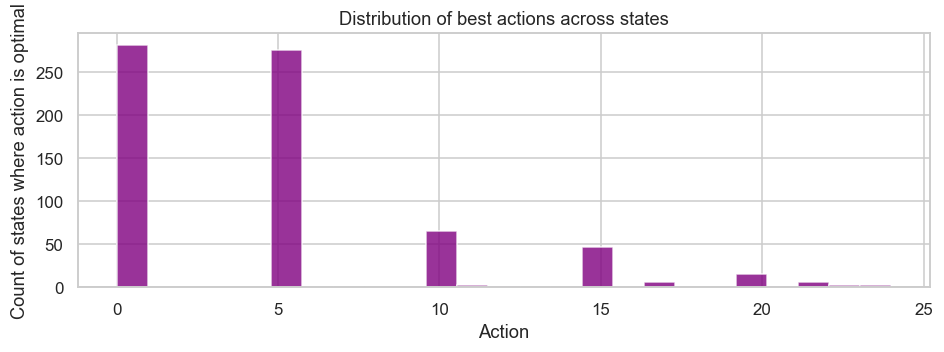
\includegraphics[width=1.0\textwidth]{best_actions_across_states.png}
    \caption{Distribution of Best Actions Across States.}
    \label{app:fig:best_actions}
\end{figure}

\begin{figure}[h]
    \centering
    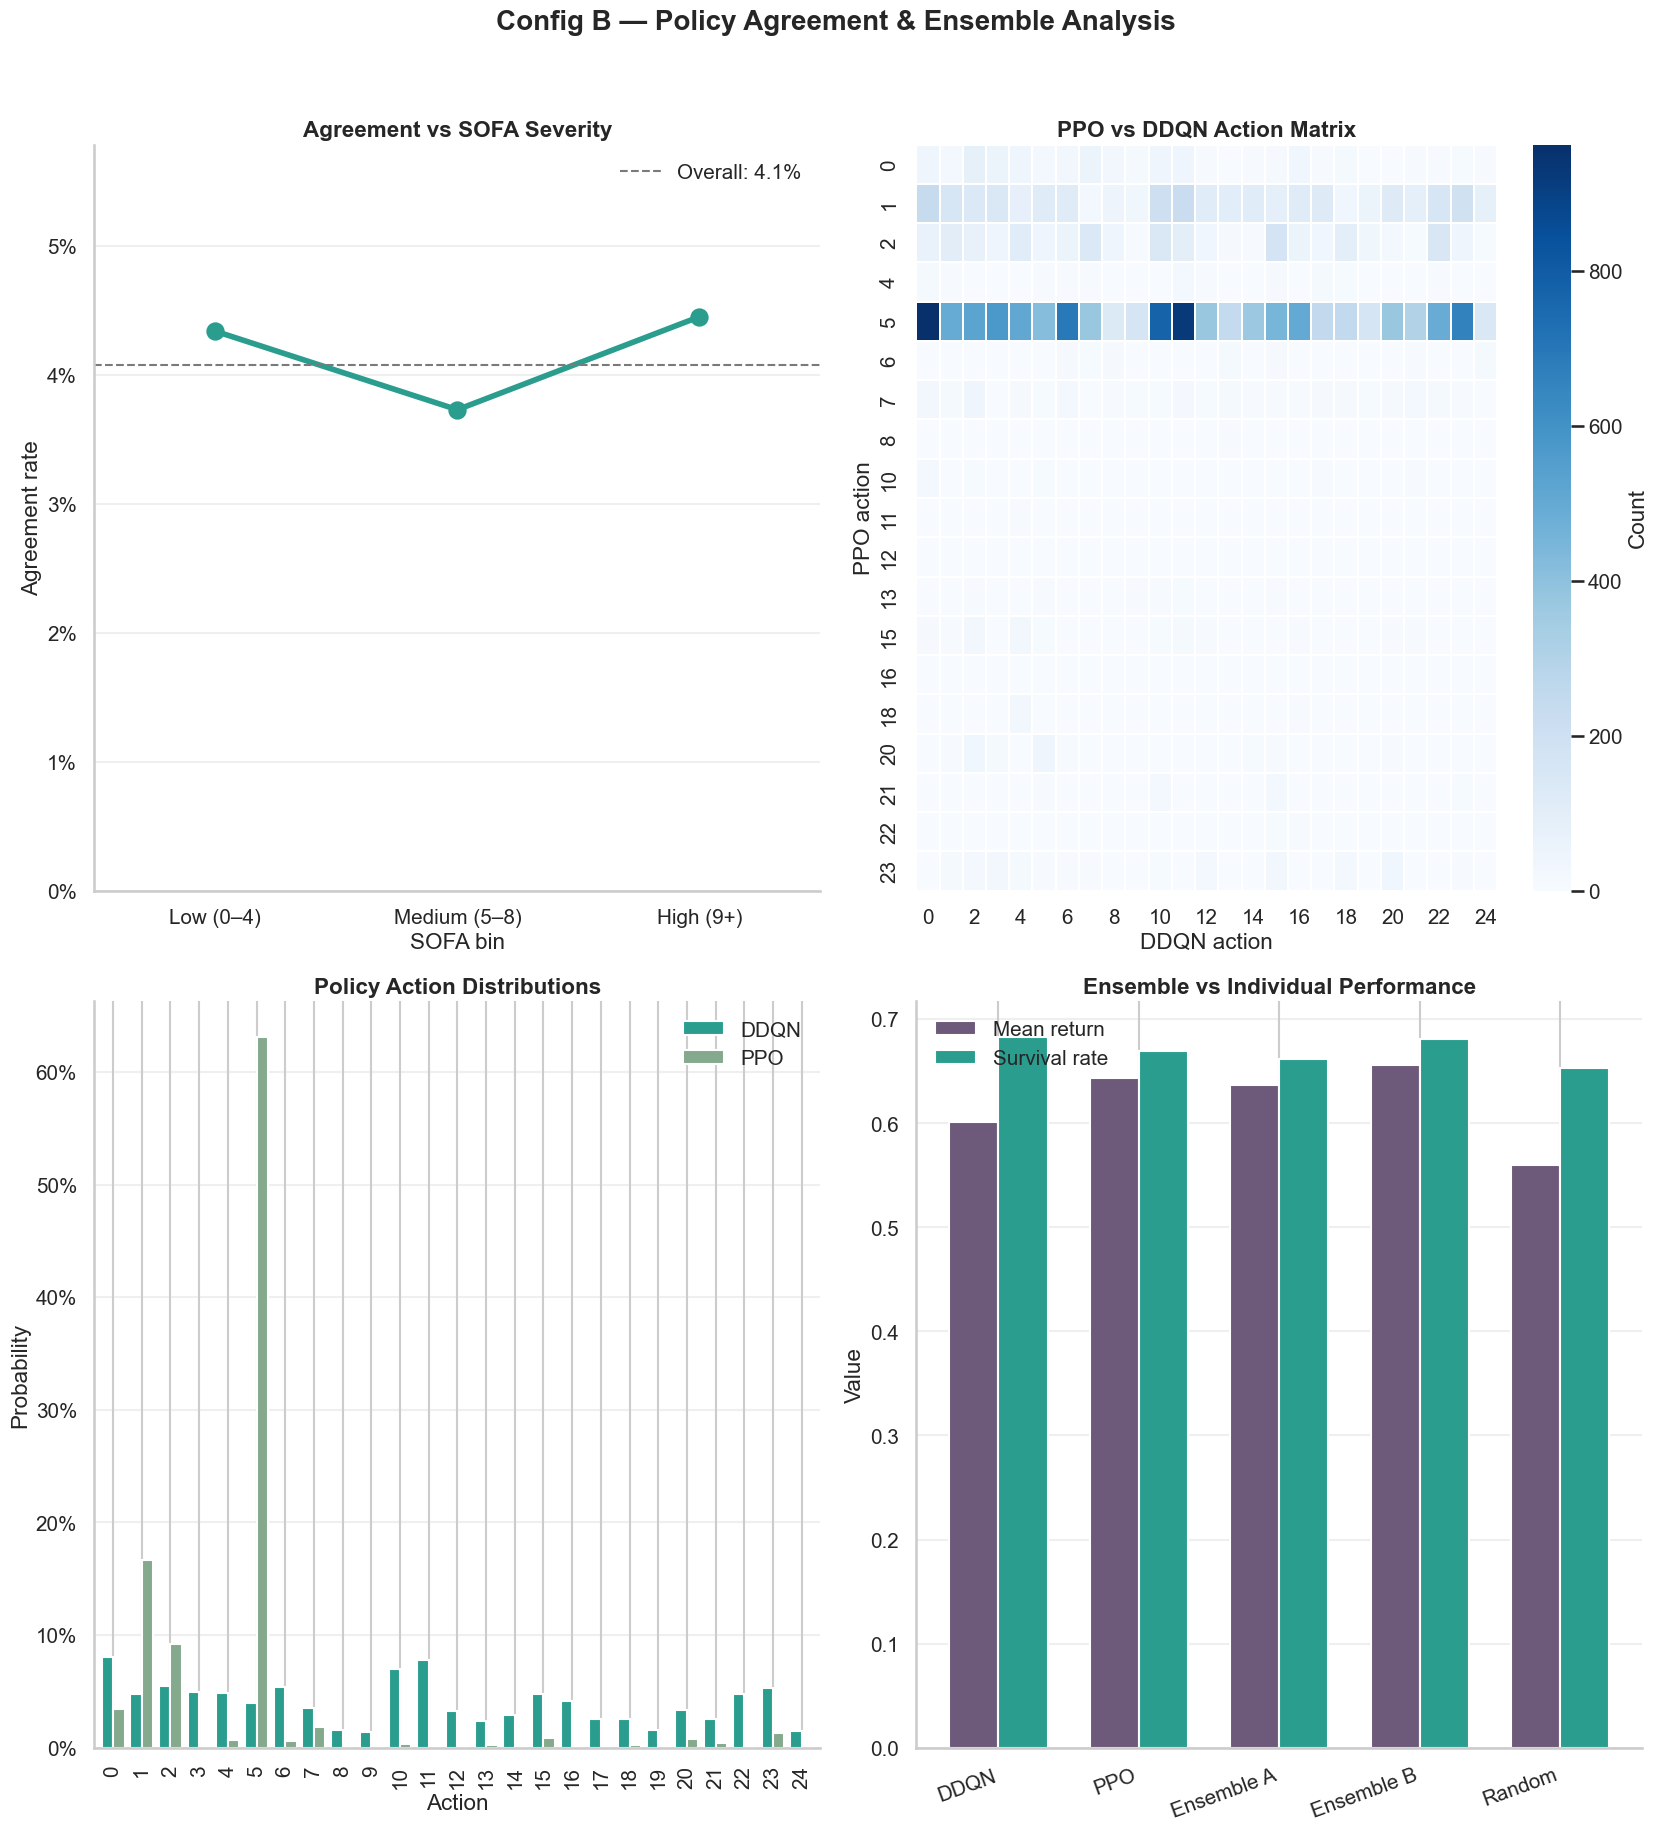
\includegraphics[width=1.0\textwidth]{policy_agreement_ensemble_analysis.png}
    \caption{Policy Agreement and Ensemble Analysis in Configuration B.}
    \label{app:fig:policy_agreement_ensemble_analysis}
\end{figure}

\clearpage
\addcontentsline{toc}{section}{References}
\bibliographystyle{plain}
\bibliography{references}

\end{document}